\documentclass[preprint,11pt]{elsarticle}
\usepackage{amsmath,amssymb}
\usepackage{graphicx}
\usepackage{booktabs}
\usepackage{longtable}
\usepackage{siunitx}
\usepackage{url}
\usepackage{caption}
\journal{Water Research}

\renewcommand{\thetable}{S\arabic{table}}
\renewcommand{\thefigure}{S\arabic{figure}}
\renewcommand{\thesection}{S\arabic{section}}

\begin{document}

\begin{frontmatter}
\title{Supporting information for\\
``Testing effort sets the water-quality criterion: an extreme-order-statistic
artefact that regulatory screening does not remove''}
\author[snu]{Jeongyun Kim}
\author[cbdri]{Jin Yoo}
\author[cbdri]{Ku Kang\corref{cor}}
\ead{bisu9082@mnd.go.kr}
\affiliation[snu]{organization={Department of Chemical and Biological Engineering, Seoul National University},
  city={Seoul}, country={Republic of Korea}}
\affiliation[cbdri]{organization={CBRN Defense Research Institute}, country={Republic of Korea}}
\cortext[cor]{Corresponding author.}
\end{frontmatter}

\tableofcontents
\clearpage

\section{Data retrieval}

\subsection{Aquatic toxicity}

ECOTOX ASCII release of 15 September 2026, downloaded from the United States
Environmental Protection Agency file service. Three files are used:
\textsf{results.txt} for the endpoint records, \textsf{tests.txt} for the
test-to-species link, and \textsf{validation/species.txt} for the taxonomy. The
result-level extract retains the endpoint codes \textsf{EC50}, \textsf{IC50},
\textsf{LC50}, \textsf{LOEC}, \textsf{LOEL}, \textsf{MATC}, \textsf{NOEC} and
\textsf{NOEL}; the \textsf{*} qualifier is stripped from endpoint strings before
matching, and records whose \textsf{conc1\_mean\_op} is one of \textsf{>},
\textsf{<}, \textsf{>=}, \textsf{<=} or \textsf{\textasciitilde} are discarded
as censored. Concentration units are converted to \si{\milli\gram\per\litre}
with the multipliers \textsf{AI mg/L} $=1$, \textsf{g/L} $=10^{3}$,
\textsf{mg/L} $=1$, \textsf{ng/L} $=10^{-6}$, \textsf{ppb} $=10^{-3}$,
\textsf{ppm} $=1$, \textsf{ug/L} $=10^{-3}$.

\subsection{Measured concentrations}

The Water Quality Portal was queried on the host
\textsf{www.waterqualitydata.us}. The characteristic-name vocabulary was
enumerated by calling the code service

\begin{quote}\small
\textsf{/Codes/characteristicname?text=<pattern>\&mimeType=json}
\end{quote}

for the patterns \textsf{perfluoro}, \textsf{fluorotelomer}, \textsf{PFOS},
\textsf{PFOA}, \textsf{sulfonamido}, \textsf{HFPO}, \textsf{polyfluoro},
\textsf{fluorobutane}, \textsf{fluorohexane}, \textsf{fluorooctane},
\textsf{fluoroheptane}, \textsf{fluorodecane} and \textsf{fluorononane}, giving
139 distinct names. Results were then requested in batches of eight names from

\begin{quote}\small
\textsf{/data/Result/search} with \textsf{mimeType=csv}, \textsf{zip=no},
\textsf{dataProfile=narrowResult}, \textsf{sampleMedia=Water},
\textsf{siteType=Stream}, \textsf{siteType=Lake, Reservoir, Impoundment},
\textsf{startDateLo=01-01-2015}
\end{quote}

returning 117\,034 results. Of these, 22\,255, or 19.0\,\%, carry a positive numeric value in
\si{\nano\gram\per\litre} or \si{\micro\gram\per\litre} with no
detection-condition flag indicating non-detection, which is the detected set
used throughout. The remainder are non-detections (89\,857 flagged as such),
quality-control results reported as percent recovery, isotopically labelled
surrogate standards, and a small number of records reporting a value of zero
together with a non-detect flag.

\section{Composition of the curated extract}

\begin{figure}[htbp]
\centering
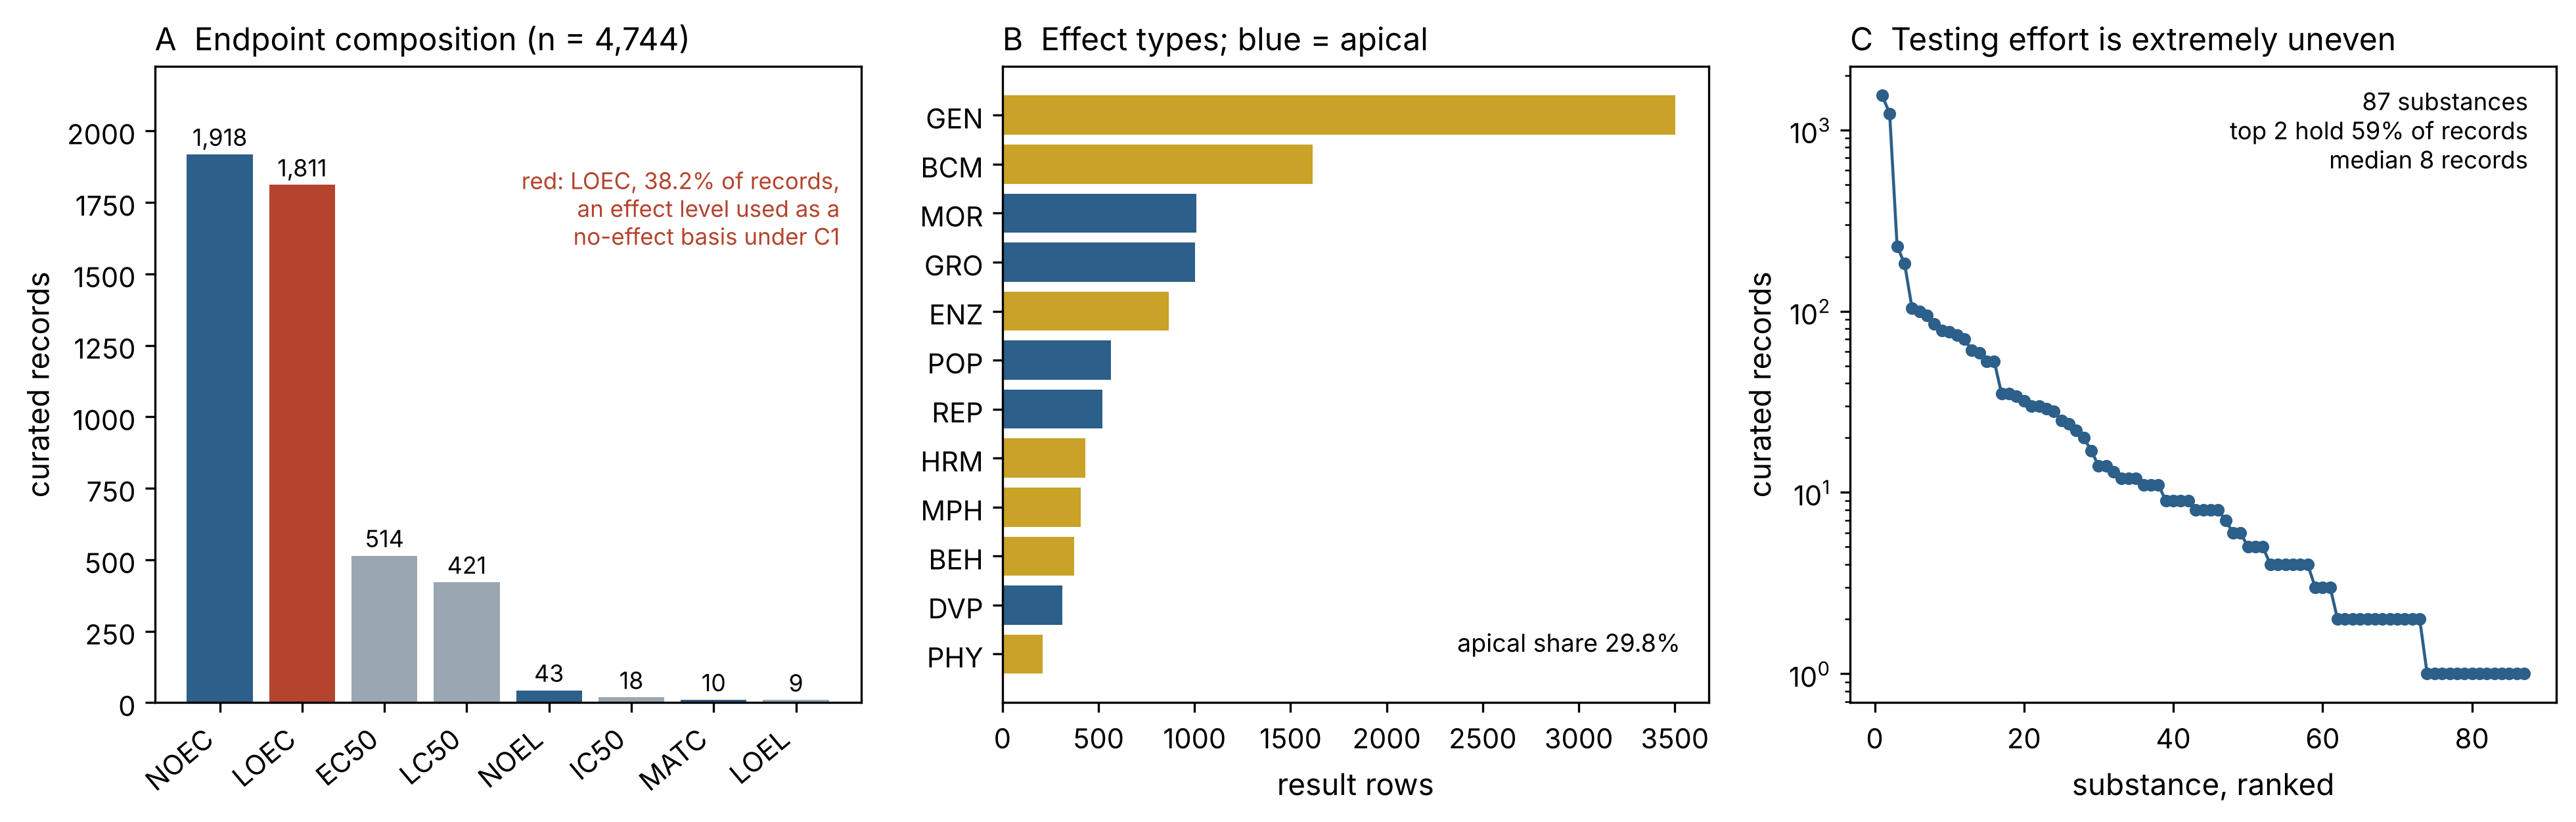
\includegraphics[width=\textwidth]{fig_01_data.png}
\caption{Composition of the curated ECOTOX extract. (A) Endpoint types; the
1811 \textsf{LOEC} records shown in red report concentrations at which an effect
was observed and enter the minimum used by convention C1. (B) Reported effect
types across result rows; blue marks the apical effects regulatory derivation
retains. (C) Curated records per substance, rank-ordered: the two most-studied
PFAS hold 59\,\% of all records and the median substance has eight.}
\label{fig:sdata}
\end{figure}

\section{Method detail}

\subsection{The regulatory-style screen}
Records were retained only if the endpoint was \textsf{NOEC}, \textsf{NOEL},
\textsf{MATC} or \textsf{EC10}; the reported effect was \textsf{MOR},
\textsf{GRO}, \textsf{REP}, \textsf{DVP} or \textsf{POP}; and
\textsf{conc1\_type} was \textsf{A} (active ingredient). Excluded effect codes
include \textsf{GEN} (gene expression), \textsf{BCM} (biochemistry),
\textsf{ENZ}, \textsf{HRM}, \textsf{BEH}, \textsf{HIS}, \textsf{CEL} and
\textsf{ACC}. Species mean chronic values are geometric means within species
and substance. The log-normal SSD is fitted by moments on the $\log_{10}$
species means and the fifth percentile taken as
$\mu + z_{0.05}\sigma$, with no further assessment factor, where five or more
species remain.

\subsection{Model experiment}
Morgan fingerprints were generated with the RDKit Morgan generator at radius 2
and 1024 bits. Random forest regressors used 150 trees and a minimum leaf size
of 3, cross-validated over five shuffled folds with a fixed seed. Three targets
were fitted independently: the minimum acute value, the median acute value and
$\log_{10}$ of the record count. Out-of-fold predictions were pooled and then
evaluated within strata of record count. The detrended fits used targets from
which an ordinary least-squares line on $\log_{10}$(records) had been
subtracted, so that any remaining fit cannot be attributed to the effort trend.

\section{Reproduction gates}

Three assertions run before any result is computed and all must pass.

\textbf{Gate 1.} The parent-level table rebuilt from the deposited record set
must reproduce a previously deposited 87-substance table exactly: equal number
of substances, equal record counts, identical minimum $\log_{10}$ toxicity, and
median acute $\log_{10}$ toxicity equal within floating-point tolerance.

\textbf{Gate 2.} The per-substance minimum $\log_{10}$ toxicity must be
recoverable from the result-level table for all 87 substances. This gate failed
at first pass with 72 of 87 reproduced. Two causes were identified and are
recorded here because they are easy to repeat: non-concentration endpoint codes
(\textsf{BCF}, \textsf{BAF}, \textsf{BMD} variants) are present in
\textsf{results.txt} and must be excluded, and the endpoint-qualifier and
censoring rules above must be applied. With both corrections the gate passes for
all 87 substances.

\textbf{Gate 3.} The generalisation set must reproduce a previously deposited
4757-chemical acute table exactly in record count, minimum and median. It passes
for all 4757 chemicals, from 106\,095 acute freshwater records.

\section{Characteristic-name to structure mapping}

Characteristic names were assigned a CAS registry number by hand. The structure
was then taken from the ECOTOX substance file keyed on that CAS, not from the
mapping table, so that the name-to-structure correspondence is checkable: if a
CAS were assigned in error, the molecular formula retrieved would not match the
name. Table~\ref{tab:s1} lists every characteristic name with quantified data
together with the formula retrieved. Acid, anionic and salt forms collapse to
one parent under the fragment-and-neutralise rule described in the main text,
so for example \textsf{Perfluorooctanoate}, \textsf{PFOA ion} and
\textsf{Perfluorooctanoic acid} all map to $\mathrm{C_8HF_{15}O_2}$.

Eighteen of the CAS numbers assigned do not appear in the ECOTOX substance file
at all. These substances are measured in United States surface water and have no
aquatic toxicity record, so no criterion can be derived for them under any
convention.

\begin{longtable}{@{}p{66mm} l r c l@{}}
\caption{Water Quality Portal characteristic names with quantified data, the CAS registry number assigned to each, the number of detections, whether that CAS appears in the ECOTOX substance file, and the molecular formula of the parent structure retrieved from ECOTOX. The formula is shown so that the name-to-structure assignment can be checked independently of the mapping table.}\label{tab:s1}\\
\toprule
Characteristic name & CAS & $n$ & in ECOTOX & parent formula \\
\midrule
\endfirsthead
\toprule
Characteristic name & CAS & $n$ & in ECOTOX & parent formula \\
\midrule
\endhead
Perfluorobutanoate & 375-22-4 & 1,557 & yes & $\mathrm{C4HF7O2}$ \\
PFOA ion & 335-67-1 & 1,501 & yes & $\mathrm{C8HF15O2}$ \\
Perfluorooctanesulfonate & 1763-23-1 & 1,417 & yes & $\mathrm{C8HF17O3S}$ \\
Perfluorobutanesulfonate & 375-73-5 & 1,361 & yes & $\mathrm{C4HF9O3S}$ \\
Perfluorohexanoate & 307-24-4 & 1,351 & yes & $\mathrm{C6HF11O2}$ \\
Perfluoropentanoate & 2706-90-3 & 1,169 & yes & $\mathrm{C5HF9O2}$ \\
Perfluorooctanoic acid & 335-67-1 & 1,168 & yes & $\mathrm{C8HF15O2}$ \\
Perfluoroheptanoate & 375-85-9 & 1,152 & yes & $\mathrm{C7HF13O2}$ \\
Perfluoroheptanoic acid & 375-85-9 & 1,028 & yes & $\mathrm{C7HF13O2}$ \\
Perfluorohexanesulfonate & 355-46-4 & 998 & yes & $\mathrm{C6HF13O3S}$ \\
Perfluorobutanesulfonic acid & 375-73-5 & 956 & yes & $\mathrm{C4HF9O3S}$ \\
Perfluorohexanoic acid & 307-24-4 & 866 & yes & $\mathrm{C6HF11O2}$ \\
Perfluorovaleric acid & 2706-90-3 & 848 & yes & $\mathrm{C5HF9O2}$ \\
Perfluorooctane sulfonic acid & 1763-23-1 & 822 & yes & $\mathrm{C8HF17O3S}$ \\
Perfluorononanoate & 375-95-1 & 800 & yes & $\mathrm{C9HF17O2}$ \\
Perfluorohexanesulfonic acid & 355-46-4 & 696 & yes & $\mathrm{C6HF13O3S}$ \\
Perfluorononanoic acid & 375-95-1 & 597 & yes & $\mathrm{C9HF17O2}$ \\
Perfluorobutanoic acid & 375-22-4 & 595 & yes & $\mathrm{C4HF7O2}$ \\
Perfluorooctanesulfonamide & 754-91-6 & 372 & yes & $\mathrm{C8H2F17NO2S}$ \\
Perfluoropentanesulfonate & 2706-91-4 & 286 & no & --- \\
Perfluorodecanoate & 335-76-2 & 283 & yes & $\mathrm{C10HF19O2}$ \\
Perfluorodecanoic acid & 335-76-2 & 256 & yes & $\mathrm{C10HF19O2}$ \\
Perfluoropentane sulfonic acid & 2706-91-4 & 247 & no & --- \\
6:2 Fluorotelomer sulfonate acid & 27619-97-2 & 153 & yes & $\mathrm{C8H5F13O3S}$ \\
Perfluorododecanoic acid & 307-55-1 & 134 & yes & $\mathrm{C12HF23O2}$ \\
3:3 Fluorotelomer carboxylic acid & 356-02-5 & 118 & no & --- \\
Perfluoroundecanoic acid & 2058-94-8 & 102 & yes & $\mathrm{C11HF21O2}$ \\
N-ethyl perfluorooctanesulfonamidoacetic acid & 2991-50-6 & 80 & no & --- \\
Perfluoro-3-methoxypropanoic acid & 377-73-1 & 80 & no & --- \\
Fluorotelomer sulfonate 8:2 & 39108-34-4 & 75 & no & --- \\
Perfluoroundecanoate & 2058-94-8 & 73 & yes & $\mathrm{C11HF21O2}$ \\
Perfluorotridecanoic acid & 72629-94-8 & 71 & yes & $\mathrm{C13HF25O2}$ \\
Perfluoro(4-methoxybutanoic) acid & 863090-89-5 & 68 & no & --- \\
Perfluorotetradecanoic acid & 376-06-7 & 68 & no & --- \\
N-methyl perfluorooctanesulfonamidoacetic acid & 2355-31-9 & 63 & no & --- \\
Fluorotelomer sulfonate 4:2 & 757124-72-4 & 62 & no & --- \\
Perfluoroheptanesulfonate & 375-92-8 & 61 & no & --- \\
4,8-Dioxa-3H-perfluorononanoic acid & 919005-14-4 & 61 & no & --- \\
Perfluoro(2-ethoxyethane)sulfonic acid & 113507-82-7 & 60 & no & --- \\
Perfluoro-1-nonanesulfonic acid & 68259-12-1 & 60 & no & --- \\
Perfluoro-3,6-dioxaheptanoic acid & 151772-58-6 & 59 & no & --- \\
3-Perfluoroheptylpropanoic acid (7:3 FTCA) & 812-70-4 & 59 & yes & $\mathrm{C10H5F15O2}$ \\
3-Perfluoropentylpropanoic acid (5:3 FTCA) & 914637-49-3 & 59 & yes & $\mathrm{C8H5F11O2}$ \\
Perfluorobutylsulfonamide & 30334-69-1 & 59 & yes & $\mathrm{C4H2F9NO2S}$ \\
Perfluorohexanesulfonamide & 41997-13-1 & 59 & yes & $\mathrm{C6H2F13NO2S}$ \\
Perfluorohexane sulfonate & 355-46-4 & 34 & yes & $\mathrm{C6HF13O3S}$ \\
N-Ethylperfluorooctanesulfonamidoacetate & 2991-50-6 & 31 & no & --- \\
N-Ethyl-N-(2-hydroxyethyl)perfluorooctanesulfonamide & 1691-99-2 & 22 & no & --- \\
2-(N-methylperfluoro-1-octanesulfonamido)-ethanol & 24448-09-7 & 20 & yes & $\mathrm{C11H8F17NO3S}$ \\
N-Methylperfluorooctanesulfonamidoacetate & 2355-31-9 & 20 & no & --- \\
Heptafluorobutyric acid\,***\,retired\,***\,use Perfluorobutanoi & 375-22-4 & 19 & yes & $\mathrm{C4HF7O2}$ \\
N-methylperfluoro-1-octanesulfonamide & 31506-32-8 & 19 & no & --- \\
Perfluorotetradecanoate & 376-06-7 & 16 & no & --- \\
Perfluorododecanoate & 307-55-1 & 12 & yes & $\mathrm{C12HF23O2}$ \\
Perfluoro(2-propoxypropanoate) & 13252-13-6 & 11 & yes & $\mathrm{C6HF11O3}$ \\
N-ethyl perfluoro-1-octanesulfonamide & 4151-50-2 & 8 & yes & $\mathrm{C10H6F17NO2S}$ \\
Perfluorotridecanoate & 72629-94-8 & 6 & yes & $\mathrm{C13HF25O2}$ \\
N-Ethyl perfluorooctane sulfonamido ethanol & 1691-99-2 & 5 & no & --- \\
Perfluorononanesulfonate & 68259-12-1 & 5 & no & --- \\
3-perfluoropentyl propanoate & 914637-49-3 & 5 & yes & $\mathrm{C8H5F11O2}$ \\
Perfluoropalmitic acid & 67905-19-5 & 3 & no & --- \\
6:2 Fluorotelomer sulfonate\,***\,retired\,***\,use 6:2 Fluorote & 27619-97-2 & 2 & yes & $\mathrm{C8H5F13O3S}$ \\
Perfluorodecanesulfonate & 335-77-3 & 2 & no & --- \\
N-Ethyl-perfluorooctane sulfonamido acetic acid & 2991-50-6 & 2 & no & --- \\
Perfluoropentanoic acid & 2706-90-3 & 2 & yes & $\mathrm{C5HF9O2}$ \\
Perfluorooctanoate (anionic form) & 335-67-1 & 1 & yes & $\mathrm{C8HF15O2}$ \\
\bottomrule
\end{longtable}


\clearpage
\section{Species sensitivity distribution diagnostics}

Table~\ref{tab:s2} and Fig.~\ref{fig:s1} give the fit for every substance with
at least five species after the regulatory-style screen. Normality is rejected
at the 5\,\% level by the Anderson--Darling statistic for 6 of 16 substances.
The worst case is $\mathrm{C_{17}H_8Cl_2F_8N_2O_3}$, where 23 species mean
chronic values include a long run of identical reported concentrations, giving a
flat central section in the quantile plot and $R^2 = 0.39$. Its fifth percentile
should not be relied on, and it does not enter the water-side analysis because
the substance is not measured in the Water Quality Portal record.

Refitting with a log-logistic distribution changes the fifth percentile by a
median of 0.12 $\log_{10}$ units and at most 0.74. Against a spread of roughly
eight orders of magnitude between conventions, the distributional form is not a
material source of the effect reported in the main text. We note that both
families are symmetric with comparable tails, so this comparison bounds the
sensitivity to distributional choice less tightly than a skewed alternative
would.

\subsection*{Uncertainty of the fifth percentile}

Table~\ref{tab:hc5ci} gives exact normal-theory 95\,\% confidence intervals
for each fifth percentile, computed as noncentral-$t$ tolerance limits. The
intervals are wide at small species counts --- up to 7.2 $\log_{10}$ units at
five species, against 0.9 at forty-seven --- and most of the point estimates
are not statistically separable from one another. This is a limitation of the
estimator rather than of our implementation, and it is the quantitative basis
for the recommendation in the main text that an HC5 fitted to a short species
list should be reported with its interval or not fitted at all. It does not
affect the correlation result: a hierarchical bootstrap that resamples species
within substances as well as substances returns
$\rho = -0.61$, 95\,\% CI $[-0.87, -0.27]$.

\begin{table}[htbp]
\centering
\footnotesize
\caption{Fifth percentiles with exact normal-theory 95\,\% confidence intervals (noncentral-$t$ tolerance limits) for every substance supporting a species sensitivity distribution after the apical and chronic-duration screen. Interval width is in $\log_{10}$ units. The point estimates are not separable from one another at small species counts, which is the reason the main text reports them to two significant figures.}
\label{tab:hc5ci}
\begin{tabular}{@{}r rrr r@{}}
\toprule
species & HC5 & lower & upper & width\\
& (\si{\nano\gram\per\litre}) & (\si{\nano\gram\per\litre}) & (\si{\nano\gram\per\litre}) & ($\log_{10}$)\\
\midrule
5 & 8.04e+03 & 82.1 & \num{3.5e+04} & 2.64\\
5 & \num{3.1e+05} & \num{1.2e+04} & \num{8.8e+05} & 1.86\\
5 & \num{2.9e+05} & 2.47e+03 & \num{1.3e+06} & 2.73\\
6 & \num{1.8e+05} & \num{2.2e+04} & \num{3.9e+05} & 1.25\\
6 & \num{3.3e+05} & \num{5.2e+04} & \num{6.5e+05} & 1.10\\
6 & \num{2.7e+04} & 427 & \num{1.2e+05} & 2.47\\
7 & 114 & 0.0303 & 3.41e+03 & 5.05\\
7 & 8.8e+03 & 94.1 & \num{5.7e+04} & 2.78\\
7 & 6.31 & \num{5.0e-05} & 807 & 7.21\\
12 & \num{3.9e+06} & \num{3.8e+05} & \num{1.3e+07} & 1.54\\
15 & 218 & 69.9 & 421 & 0.78\\
34 & \num{1.1e+04} & 2.09e+03 & \num{3.7e+04} & 1.25\\
47 & 3.5e+03 & 918 & 9.46e+03 & 1.01\\
\bottomrule
\end{tabular}
\end{table}


\begin{table}[htbp]\centering\caption{Fit diagnostics for every species sensitivity distribution with at least five species. HC5 values are $\log_{10}$ of the fifth percentile in \si{\milli\gram\per\litre}. Anderson--Darling is compared with its 5\,\% critical value.}\label{tab:s2}\footnotesize\setlength{\tabcolsep}{3.4pt}
\begin{tabular}{@{}l r r r r r l r r r r@{}}\toprule
Substance & $n$ & mean & s.d. & AD & crit & normality & Shapiro $p$ & HC5 ln & HC5 ll & $\Delta$ \\\midrule
PFOS & 57 & -0.07 & 1.37 & 1.07 & 0.74 & reject & 0.017 & -2.32 & -2.33 & -0.00 \\
PFOA & 39 & 0.34 & 1.44 & 1.03 & 0.74 & reject & 0.015 & -2.02 & -2.05 & -0.03 \\
$\mathrm{C17H8Cl2F8N2O3}$ & 23 & -2.55 & 1.06 & 5.53 & 0.72 & reject & 0.000 & -4.29 & -3.54 & +0.74 \\
$\mathrm{C2HF3O2}$ & 14 & 2.02 & 1.06 & 1.03 & 0.71 & reject & 0.007 & 0.28 & 0.64 & +0.36 \\
PFBS & 10 & 0.16 & 2.94 & 0.57 & 0.69 & ok & 0.127 & -4.68 & -4.80 & -0.12 \\
HFPO-DA & 9 & -0.39 & 1.79 & 0.43 & 0.68 & ok & 0.175 & -3.33 & -3.32 & +0.00 \\
$\mathrm{C23H22F7IN2O4S}$ & 8 & -0.60 & 1.12 & 0.70 & 0.67 & reject & 0.047 & -2.44 & -2.39 & +0.05 \\
PFHxS & 8 & -0.49 & 0.82 & 0.96 & 0.67 & reject & 0.008 & -1.84 & -1.60 & +0.23 \\
$\mathrm{C12H2F20O2}$ & 7 & 0.11 & 0.53 & 0.38 & 0.65 & ok & 0.523 & -0.76 & -0.63 & +0.13 \\
$\mathrm{C12H3F21O2}$ & 7 & 0.05 & 0.94 & 0.28 & 0.65 & ok & 0.613 & -1.50 & -1.37 & +0.13 \\
$\mathrm{C10H3F17O2}$ & 6 & 0.12 & 0.44 & 0.20 & 0.63 & ok & 0.886 & -0.61 & -0.61 & +0.00 \\
PFNA & 5 & -0.61 & 0.90 & 0.25 & 0.61 & ok & 0.723 & -2.09 & -1.88 & +0.21 \\
PFBA & 5 & 0.83 & 2.38 & 0.36 & 0.61 & ok & 0.293 & -3.09 & -2.90 & +0.20 \\
$\mathrm{C10H2F16O2}$ & 5 & 0.39 & 0.55 & 0.38 & 0.61 & ok & 0.261 & -0.51 & -0.34 & +0.17 \\
$\mathrm{C8H3F13O2}$ & 5 & 0.78 & 0.81 & 0.28 & 0.61 & ok & 0.473 & -0.54 & -0.48 & +0.06 \\
6:2 FTS & 5 & 0.41 & 0.94 & 0.28 & 0.61 & ok & 0.552 & -1.14 & -1.12 & +0.02 \\
\bottomrule\end{tabular}\end{table}


\begin{figure}[htbp]
\centering
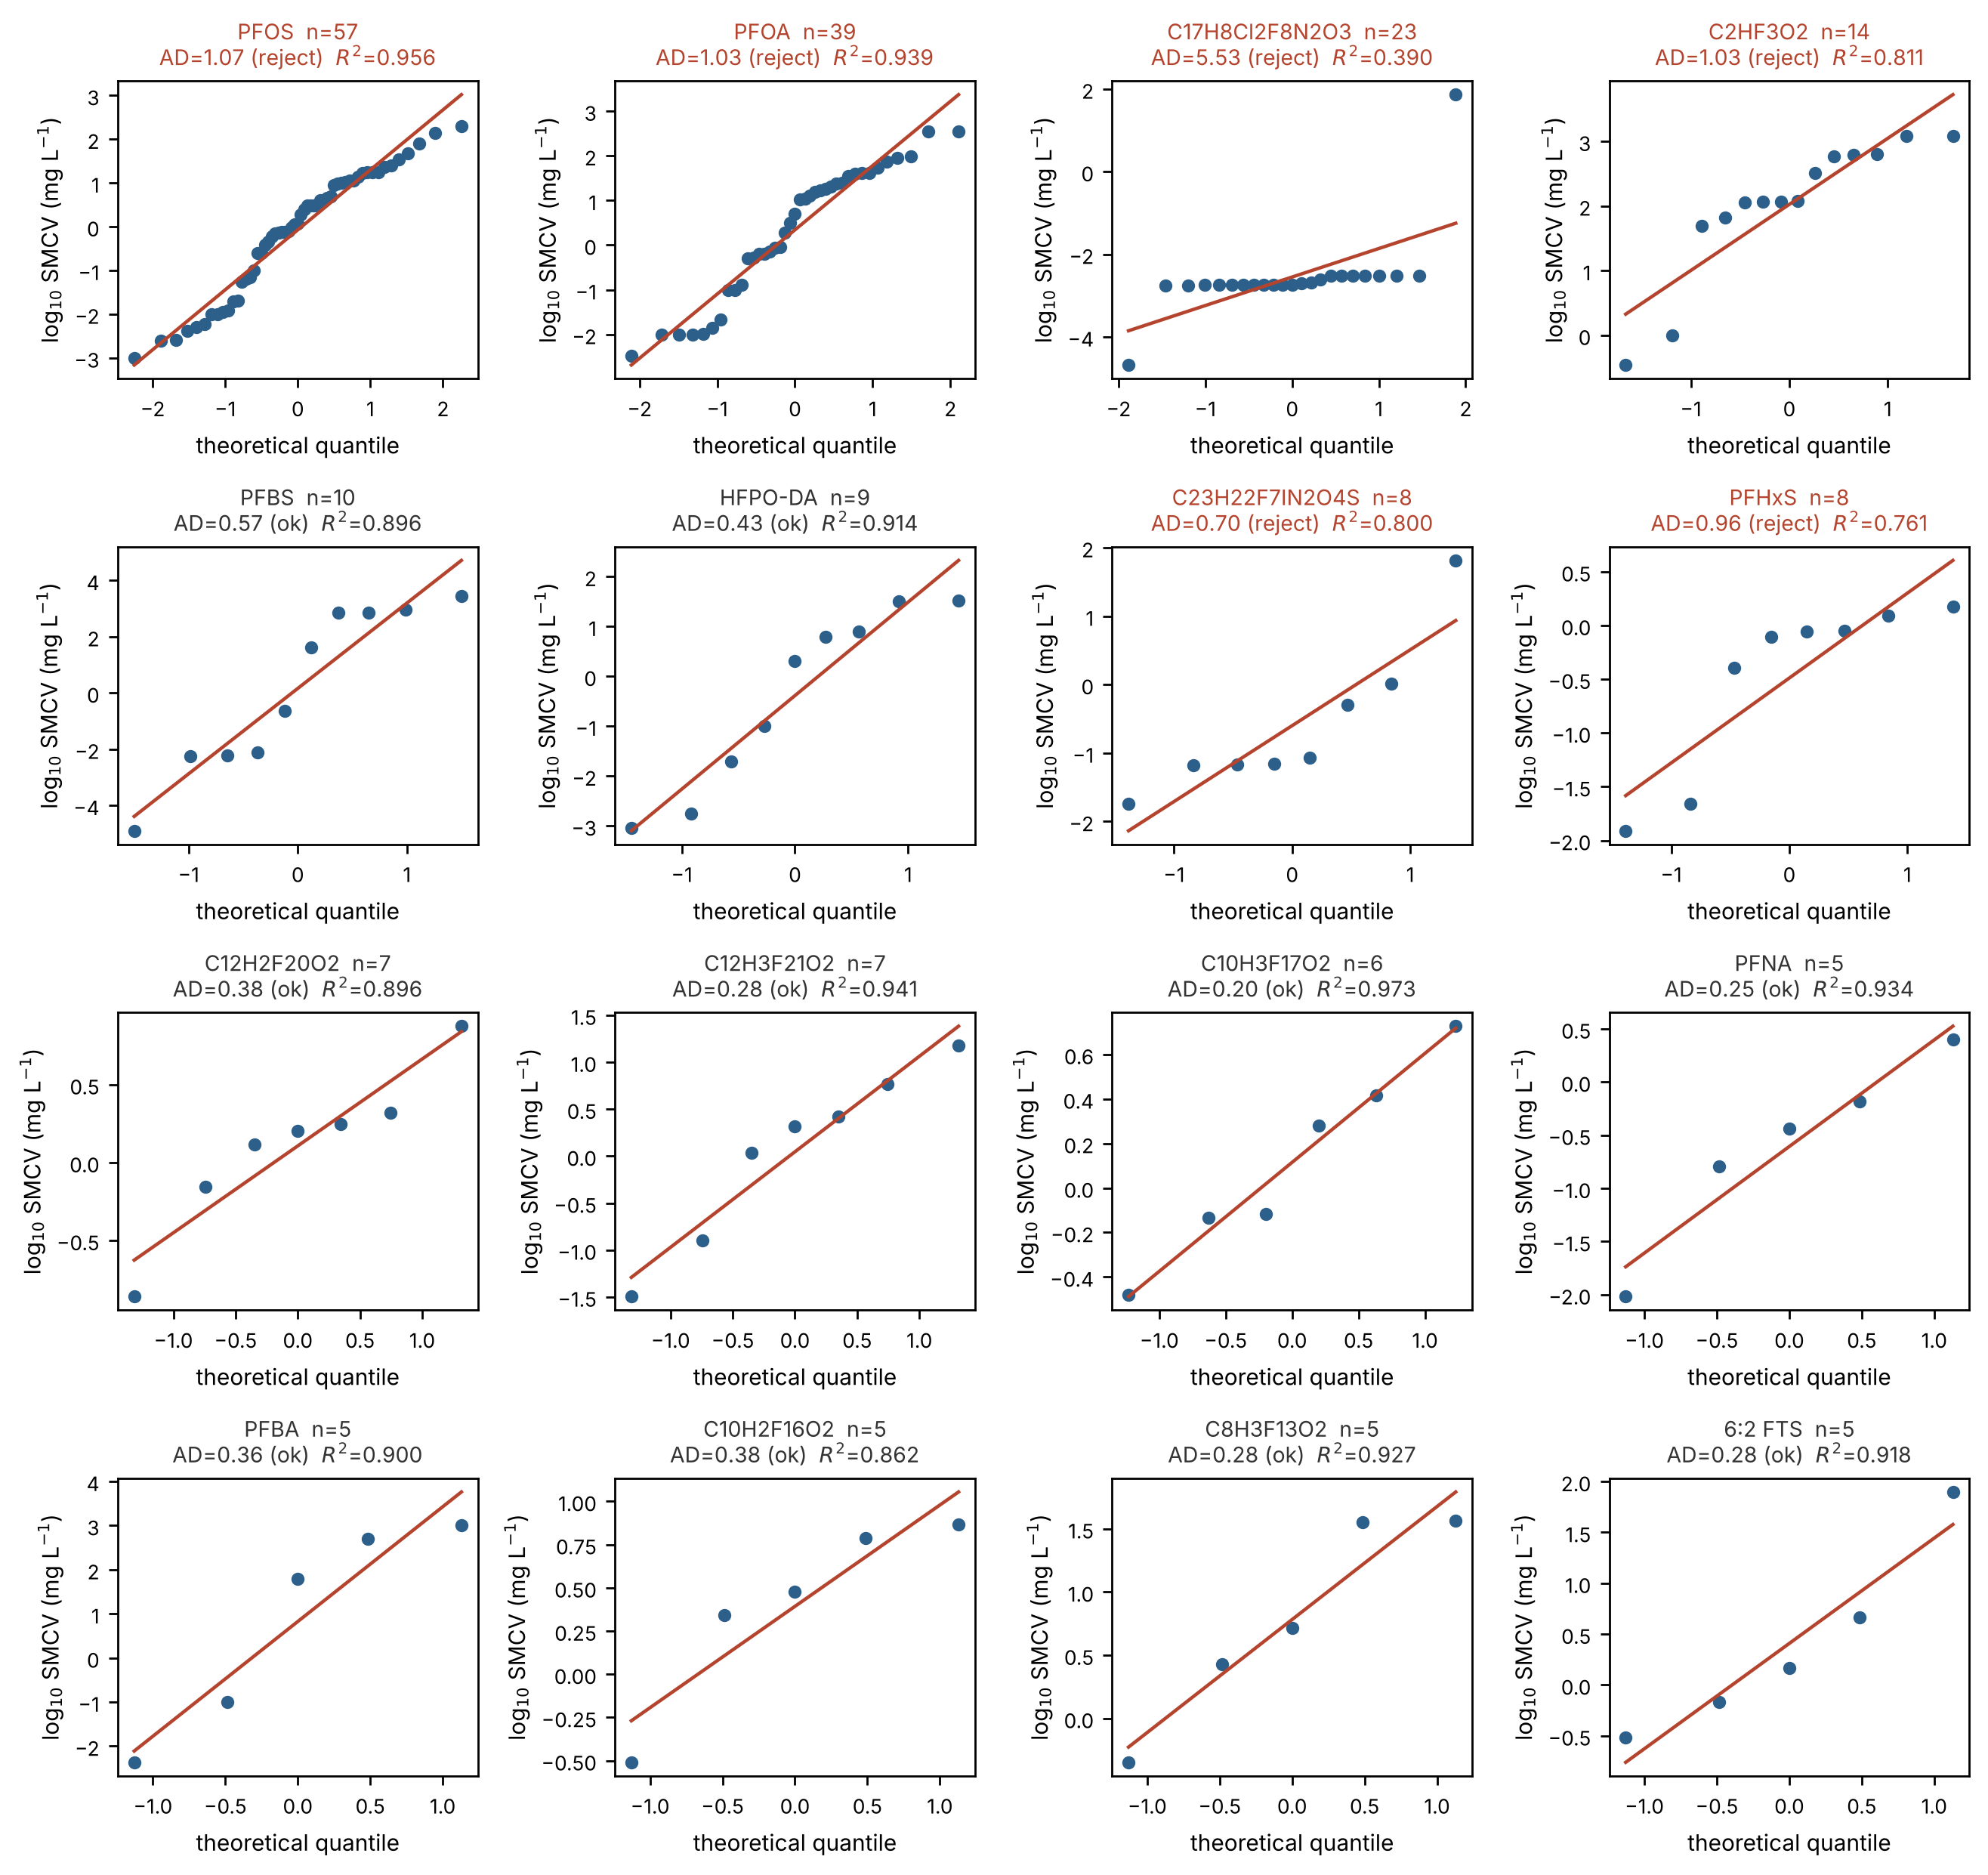
\includegraphics[width=\textwidth]{fig_si_qq.png}
\caption{Normal quantile plots of species mean chronic values for every
substance with at least five species after the screen, ordered by species count.
Red titles mark substances for which normality is rejected at the 5\,\% level.
Substances without a common abbreviation are labelled by the molecular formula
of the parent structure.}
\label{fig:s1}
\end{figure}

\clearpage
\section{Sensitivity of the effort correlation}

The central result of the main text is that the Spearman correlation between
$\log_{10}$ of the number of curated records and the derived criterion remains
negative after the regulatory screen. Table~\ref{tab:s3} varies the two choices
that define the distribution step.

\begin{table}[htbp]
\centering
\caption{Spearman correlation between testing effort and the SSD fifth
percentile, under varying minimum species requirements and distributional form.
Bootstrap 95\,\% confidence intervals from 4000 resamples.}
\label{tab:s3}
\begin{tabular}{@{}l l r r l@{}}
\toprule
Minimum species & Distribution & substances & $\rho$ & 95\,\% CI \\
\midrule
3  & log-normal    & 24 & $-0.666$ & $[-0.898, -0.337]$ \\
5  & log-normal    & 16 & $-0.691$ & $[-0.944, -0.312]$ \\
5  & log-logistic  & 16 & $-0.700$ & $[-0.952, -0.324]$ \\
8  & log-normal    &  8 & $-0.286$ & $[-0.905, +0.615]$ \\
10 & log-normal    &  5 & $-0.100$ & $[-1.000, +1.000]$ \\
\bottomrule
\end{tabular}
\end{table}

The correlation is stable in sign and magnitude for minimum species
requirements of three and five and for either distributional form. At eight and
ten species the estimate is uninformative: raising the requirement removes the
data-poor substances, which is to say it removes the variation in effort that
the correlation is measuring, and leaves eight and five substances
respectively. We report these rows rather than omitting them, because the
collapse is itself the point --- a stricter data requirement does not correct the
artefact, it removes the ability to observe it while leaving the data-poor
substances to be assessed by some other route.

\section{Exceedance over all results}

Exceedance fractions in the main text are computed over detections. The Water
Quality Portal returns 117\,034 results for the characteristic names queried, of
which 19.0\,\% are detections. Table~\ref{tab:s4} gives both views.
The ordering of conventions is identical; the absolute fractions fall by a
factor of about three.

We do not impute substituted values for non-detections. The
\textsf{narrowResult} profile we queried does not carry the reporting-limit
value, so a non-detection in this extract cannot be placed relative to a
criterion. This is a limitation of our query rather than of the archive: the
\textsf{resultPhysChem} profile carries
\textsf{DetectionQuantitationLimitMeasure}, and a detection-limit URL is
populated for 53\,399 of the 117\,034 results we retrieved. A reanalysis that
recovers those limits would allow each non-detection to be classified as
certainly compliant, certainly exceeding, or undetermined, and would replace
the two bounding columns reported here with a proper interval. We flag this as
the single most useful extension of the monitoring side of this work. This matters most for the conventions whose criteria
are lowest. The median C1 criterion of \SI{0.05}{\nano\gram\per\litre} lies
below the first percentile of all detected concentrations in this dataset
(\SI{0.21}{\nano\gram\per\litre}); only 4 of 20\,682 detections fall below
it. For PFOA and PFOS the C1 criterion is \SI{0.001}{\nano\gram\per\litre}
and no detection anywhere in the record falls below it. Under that convention
the compliance status of a non-detecting sample is therefore not determined by
the measurement, which is a property of the criterion rather than of the
monitoring.

\begin{table}[htbp]\centering\caption{Exceedance computed over detections only, as reported in the main text, and over all returned Water Quality Portal results for the same substances, with non-detections counted as not exceeding. The latter is a lower bound: reporting limits are not carried in the result profile used, so a non-detection cannot be placed relative to a criterion that lies below the limit.}\label{tab:s4}\footnotesize
\begin{tabular}{@{}l r r r r@{}}\toprule
Convention & detections & all results & \% of detections & \% of all \\\midrule
lowest, all endpoints (as published) & 20,682 & 63,791 & 76.50 & 24.80 \\
lowest, LOECs removed & 20,682 & 63,791 & 76.04 & 24.65 \\
lowest acute & 18,104 & 47,913 & 22.70 & 8.58 \\
median acute, record-resolved & 18,104 & 47,913 & 0.11 & 0.04 \\
median acute, species-resolved & 18,104 & 47,913 & 0.11 & 0.04 \\
lowest chronic NOEC, EU-TGD AF & 20,480 & 60,463 & 55.53 & 18.81 \\
lowest apical chronic SMCV, AF 10 & 20,539 & 60,590 & 8.48 & 2.88 \\
SSD HC5 of apical chronic SMCVs & 12,688 & 29,328 & 0.78 & 0.34 \\
\bottomrule\end{tabular}\end{table}


\section{Assessment-factor compensation}

The main text reports that the EU Technical Guidance assessment factor supplies
14\,\% of the compensation the effort dependence would require. The calculation
is a decomposition of three ordinary least-squares slopes against
$\log_{10}$(records), over the 62 substances that have both a chronic
\textsf{NOEC} and a factor:

\begin{table}[htbp]
\centering
\caption{Decomposition of the effort dependence of the EU-TGD criterion. Because
the criterion is the numerator divided by the factor, the three slopes satisfy
$-1.821 = -2.123 - (-0.302)$ exactly.}
\label{tab:s5}
\begin{tabular}{@{}l r r@{}}
\toprule
Quantity & slope per decade of records & $p$ \\
\midrule
$\log_{10}$ lowest chronic \textsf{NOEC} & $-2.123$ & $1.9\times10^{-10}$ \\
$\log_{10}$ assessment factor            & $-0.302$ & $1.4\times10^{-9}$ \\
$\log_{10}$ derived criterion            & $-1.821$ & $2.0\times10^{-8}$ \\
\bottomrule
\end{tabular}
\end{table}

The factor takes three values in this dataset (10 for 7 substances, 50 for 22,
100 for 33), a range of one $\log_{10}$ unit. The lowest chronic \textsf{NOEC}
spans 9.2 $\log_{10}$ units over the same substances. For the factor to absorb
the effort dependence it would have to vary over roughly seven decades rather
than one.

\section{Reporting discretisation in the monitoring record}

Measured PFAS concentrations are reported on a coarse numerical grid. Among the
20\,682 detections joined to a criterion, 2295 distinct values occur; 66.2\,\%
fall exactly on a \SI{0.1}{\nano\gram\per\litre} grid, 48.4\,\% are reported to
two significant figures and 14.4\,\% to one. The ten commonest values account
for 14.1\,\% of all detections. The record is drawn from many organisations, the
largest contributing 24.6\,\% of detections, so the discretisation reflects
general laboratory reporting practice rather than one source.

This is visible in the main text: PFOS and PFOA have the same median detected
concentration to two decimal places, \SI{3.50}{\nano\gram\per\litre}. With 2239
and 2670 detections on a common grid, and only 17 and 18 observations sitting
exactly at their respective medians, the coincidence follows from two similar
distributions being rounded the same way rather than from a shared artefact.

The discretisation does not affect the exceedance results, because every
criterion compared against these values sits either far below or far above the
grid spacing. Re-evaluating exceedance with the measured values perturbed by
independent multiplicative noise of $\pm 10\,\%$, over 200 replicates, moves the
C1 figure from 76.50\,\% to a mean of 76.52\,\% with a 95\,\% range of
$[76.45, 76.59]$.

\clearpage
\section{Robustness of the effort correlation}

Table~\ref{tab:rob} collects the checks bearing on alternative explanations for
the correlation. None removes it.

\begin{table}[htbp]
\centering\footnotesize
\caption{Robustness checks on the correlation between testing effort and the
derived criterion. Partial correlations control the stated variable.}
\label{tab:rob}
\begin{tabular}{@{}l rrr@{}}
\toprule
check & C6$'$ & C7a & C7b\\
\midrule
as reported & $-0.590$ & $-0.609$ & $-0.681$\\
partial, controlling carbon number & $-0.597$ & $-0.627$ & $-0.674$\\
effort as distinct tests, not result rows & $-0.599$ & $-0.626$ & $-0.710$\\
excluding three non-OECD-PFAS parents & $-0.590$ & $-0.609$ & $-0.681$\\
bootstrap 95\,\% CI (5000 draws) & $[-0.82,-0.25]$ & $[-0.82,-0.29]$ & $[-0.91,-0.28]$\\
\bottomrule
\end{tabular}
\end{table}

Chain length is the obvious confounder in a PFAS dataset, since longer chains
are both more toxic and more studied. It is not operating here: $\rho$ between
carbon number and $\log_{10}$ records is $-0.12$ to $-0.25$ depending on the
convention, and controlling for it leaves every correlation within 0.02 of its
raw value.

For the thirteen-substance SSD set a permutation null was computed by shuffling
the fifth percentiles against record count 20\,000 times. The null has mean
$+0.00$ and standard deviation $0.29$, with a 95\,\% band of $[-0.56, +0.55]$;
the observed $-0.681$ gives $P = 0.0068$.

On the monitoring side, exceedance is insensitive to which organisations
contributed the data. The largest single contributor supplies 24.6\,\% of joined
detections; removing each of the eight largest in turn moves the C1 sample
exceedance between 22.1\,\% and 26.1\,\% against 24.2\,\% for the full set, and
weighting one median value per station and substance gives 22.9\,\%.

\clearpage
\section{Model experiment}


A growing literature trains QSAR and machine-learning models to predict aquatic
criteria or lowest-observed toxicity values for untested PFAS
\cite{khan2019ecotoxqsar, sarkar2026pfasqsar, liang2025datagaps}. We tested what
the artefact does to such a model: random forests on Morgan fingerprints of the
4311 broad-set chemicals with a parsable structure, five-fold cross-validated,
with the minimum and the median acute value as alternative targets.

We expected a model fitted to the minimum to learn the effort component, and it
does not. Structure predicts record count weakly by $R^2$ ($0.085$) though not
negligibly by rank (Spearman $\rho = +0.316$), and
removing the effort trend from the target before fitting changes aggregate
performance by two to three percent either way. The model cannot learn the
component, because record count is not a structural property and is not among
its inputs. The consequence is worse. The minimum-target model predicts a
typical minimum from structure while the true minimum has been pushed downward
by sampling depth to an extent the model cannot see, so its bias runs with
effort: it under-predicts by 0.66 $\log_{10}$ units for chemicals with a single
record and \emph{over}-predicts by 2.33 for chemicals with a hundred or more, a
swing of 3.0 orders of magnitude (Fig.~\ref{fig:simodel}). The median-target model
swings by 0.47. Aggregate $R^2$ for the minimum target is 0.371, concealing $R^2 = -0.951$ in
the most-studied stratum ($n = 169$), where the model is worse than predicting
that stratum's mean. Stratum $R^2$ is normalised by the variance within the
stratum and is not comparable across strata; the bias figures, in $\log_{10}$
units, carry the argument. The bias pattern is in part arithmetically
guaranteed: with record count absent from the inputs, a structure-only model
predicts an average over the record-count distribution and must under-predict
where the target is low and over-predict where it is high. That it is
guaranteed is the point --- it applies to every structure-only model of an
extreme-anchored target, not only to this one.

The direction matters for safety: for the best-studied chemicals the model says
the most sensitive endpoint lies two orders of magnitude higher, that is less
hazardous, than the database records. The failure is also invisible to the
metric such studies most often report, since Spearman $\rho$ within each stratum
stays between 0.57 and 0.63 for the minimum target --- the ranking survives
while the calibration does not. Predictive toxicology has approached this
requirement from other directions, through applicability-domain analysis
\cite{sahigara2012ad}, out-of-distribution alerting \cite{kang2026openset} and
benchmark design that separates architecture from dataset artefacts
\cite{kim2026driftrobust}, but none catches this failure, because training and
test sets carry the bias equally. What catches it is stratifying performance by
each substance's training support and reporting an error metric sensitive to
level rather than rank. Mechanistic anchoring of the endpoint avoids the problem
rather than detecting it \cite{jang2025opqsar}.

\begin{figure}[htbp]
\centering
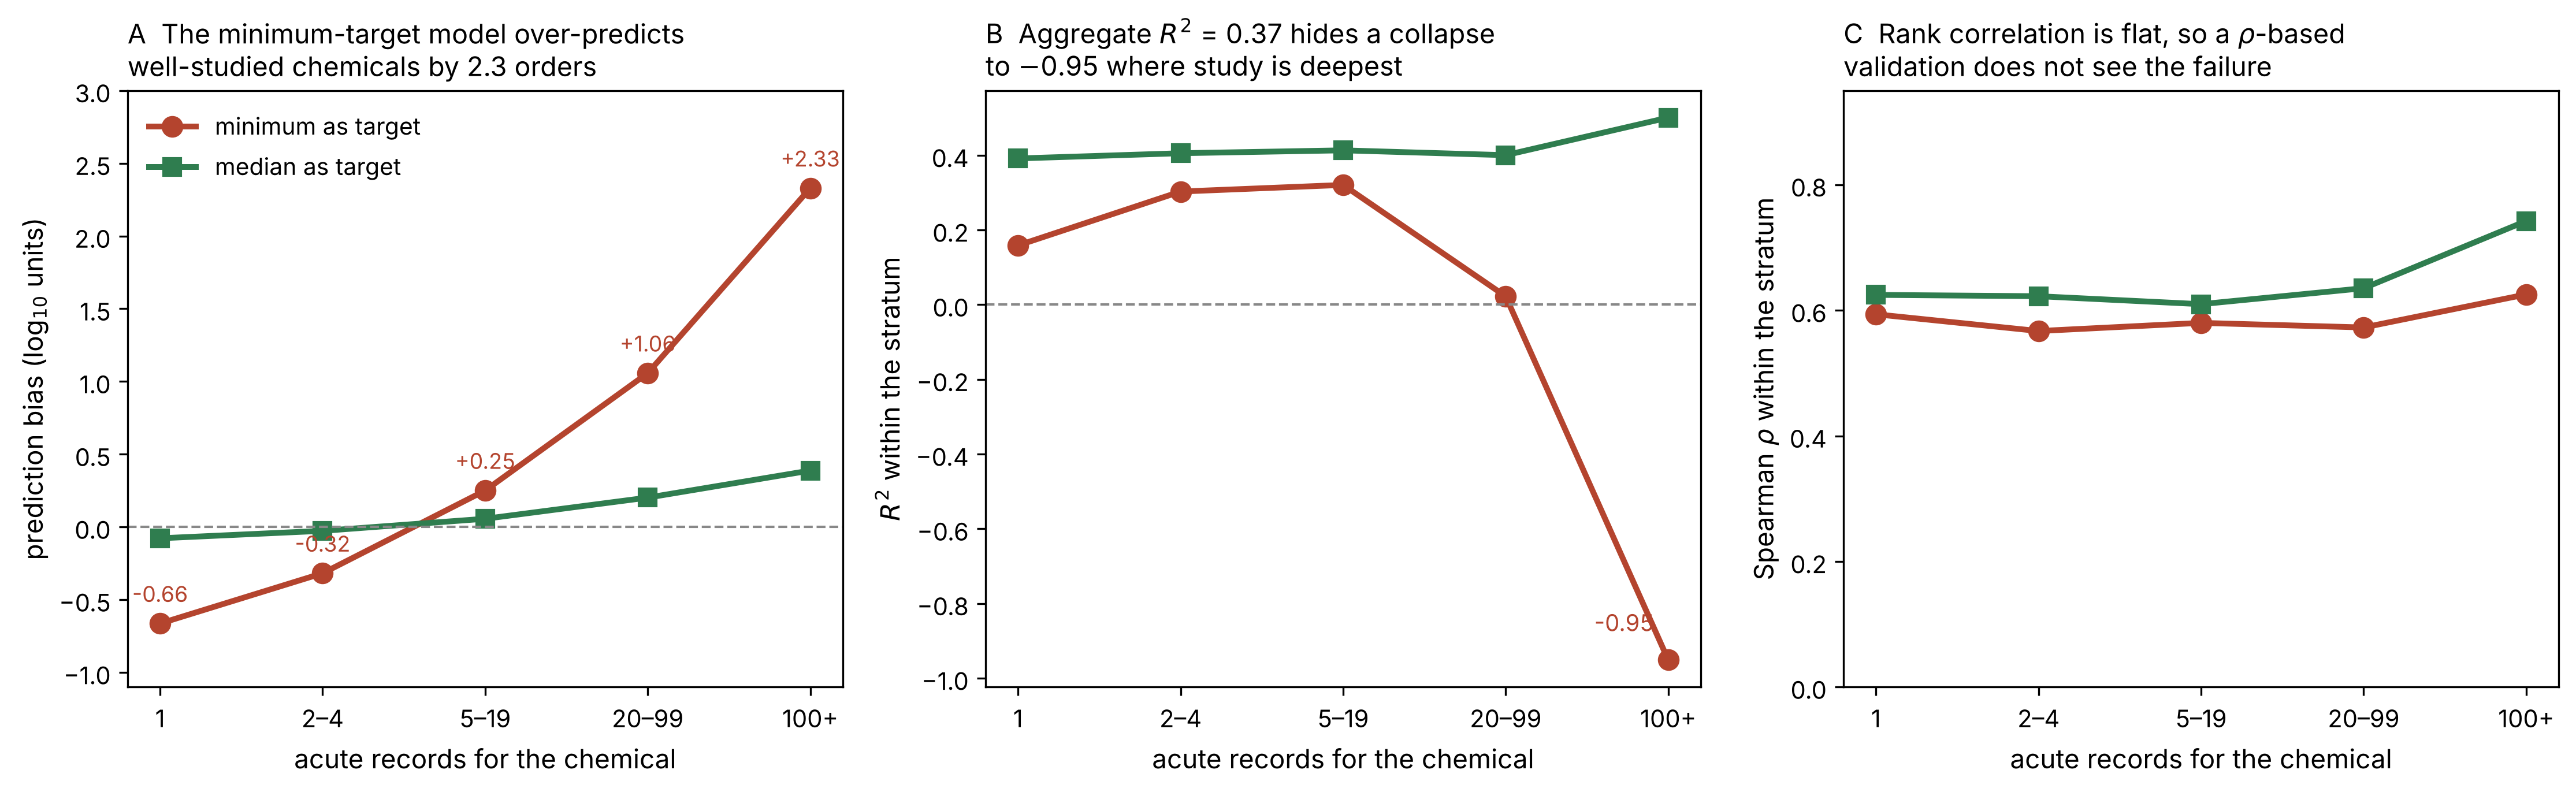
\includegraphics[width=\textwidth]{fig_07_model.png}
\caption{Random forests on Morgan fingerprints of 4311 ECOTOX chemicals,
five-fold cross-validated, with the minimum and the median acute value as
alternative targets, evaluated within strata of record count. (A) Prediction
bias. (B) Coefficient of determination. (C) Spearman correlation.}
\label{fig:simodel}
\end{figure}


\clearpage
\section{Per-substance results}

Table~\ref{tab:persub} gives the derived criterion and the exceedance fraction
for every substance measured in the monitoring record.

\begin{table}[p]
\centering
\caption{Measured concentrations, derived criteria and exceedance by substance.
Measurements are Water Quality Portal results for United States stream and lake
stations, 2016--2026. Criteria are in \si{\nano\gram\per\litre}: C1 the lowest
value over all endpoints with an assessment factor of 1000, C6 the lowest
chronic \textsf{NOEC} with an EU Technical Guidance factor, C7b the fifth
percentile of a log-normal species sensitivity distribution fitted to apical
chronic species mean values. A dash means the convention cannot be applied for
want of qualifying data.}
\label{tab:persub}
\scriptsize
\setlength{\tabcolsep}{3.2pt}
\begin{tabular}{@{}l r r r r r r r r r r@{}}
\toprule
 & \multicolumn{3}{c}{measured} & tox & \multicolumn{3}{c}{criterion (\si{\nano\gram\per\litre})}
 & \multicolumn{3}{c}{\% samples $>$ criterion} \\
\cmidrule(lr){2-4}\cmidrule(lr){6-8}\cmidrule(lr){9-11}
Substance & $n$ & sites & median & recs & C1 & C6 & C7b & C1 & C6 & C7b \\
\midrule
PFOA & 2,670 & 1013 & 3.50 & 1,232 & 0.001 & 0.1 & 9,516 & 100.00 & 99.96 & 0.00 \\
PFBS & 2,317 & 892 & 2.86 & 183 & 0.005 & 1 & 21 & 100.00 & 76.18 & 4.01 \\
PFOS & 2,239 & 876 & 3.50 & 1,548 & 0.001 & 0.1 & 4,738 & 100.00 & 99.91 & 0.22 \\
PFHxA & 2,217 & 856 & 3.50 & 78 & 0.2 & 4 & --- & 100.00 & 45.60 & --- \\
PFHpA & 2,180 & 821 & 1.67 & 11 & 7.2 & 144 & --- & 6.28 & 0.55 & --- \\
PFBA & 2,171 & 867 & 4.96 & 70 & 0.05 & 1 & 807 & 100.00 & 97.56 & 0.05 \\
PFPeA & 2,019 & 852 & 4.00 & 9 & 7.17 & 143 & --- & 31.40 & 0.84 & --- \\
PFHxS & 1,728 & 699 & 1.80 & 59 & 0.445 & 8.9 & \num{1.46e+04} & 92.82 & 11.52 & 0.00 \\
PFNA & 1,397 & 591 & 1.30 & 104 & 0.02 & 0.4 & 8,154 & 100.00 & 90.19 & 0.00 \\
PFDA & 539 & 216 & 0.87 & 30 & 1 & 20 & --- & 39.70 & 0.37 & --- \\
FOSA & 372 & 188 & 0.51 & 8 & 1.15 & 11.5 & --- & 16.67 & 5.91 & --- \\
PFUnA & 175 & 76 & 1.04 & 14 & 9.32 & 186 & --- & 2.86 & 1.14 & --- \\
6:2 FTS & 155 & 67 & 7.90 & 30 & 1.7 & 100 & \num{7.30e+04} & 82.58 & 3.23 & 0.00 \\
PFDoA & 146 & 31 & 2.00 & 25 & 9.89 & 198 & --- & 9.59 & 2.74 & --- \\
PFTrDA & 77 & 25 & 2.00 & 12 & 10 & 100 & --- & 2.60 & 0.00 & --- \\
5:3 FTCA & 64 & 11 & 8.00 & 2 & \num{2.25e+04} & --- & --- & 0.00 & --- & --- \\
7:3 FTCA & 59 & 10 & 8.00 & 5 & 400 & --- & --- & 0.00 & --- & --- \\
FBSA & 59 & 10 & 0.80 & 9 & 121 & 1,210 & --- & 0.00 & 0.00 & --- \\
FHxSA & 59 & 10 & 0.80 & 11 & 100 & --- & --- & 0.00 & --- & --- \\
N-MeFOSE & 20 & 5 & 69.55 & 1 & \num{1.35e+06} & --- & --- & 0.00 & --- & --- \\
HFPO-DA & 11 & 10 & 3.20 & 85 & 0.01 & 1 & 472 & 100.00 & 100.00 & 0.00 \\
N-EtFOSA & 8 & 4 & 24.35 & 35 & 87 & \num{1.00e+04} & --- & 0.00 & 0.00 & --- \\
\bottomrule
\end{tabular}
\end{table}

\section{Software}

Analysis in Python 3.13 with pandas, NumPy, SciPy and RDKit. Parent structures
are produced with \textsf{rdMolStandardize.Uncharger} applied to the largest
fluorine-containing fragment, canonicalised with \textsf{MolToSmiles}. Figures
with Matplotlib. Bibliographic metadata for every added reference was retrieved
from the Crossref REST API rather than transcribed, so that author lists,
volumes and page ranges are taken from the publisher record.

\clearpage
\bibliographystyle{elsarticle-num}
\bibliography{myref}

\end{document}
